\chapter{Implementation}
\label{ch:implementation}


\section{Technical and Architectural Aspects}
\subsection{Publish–subscribe pattern}

\section{Deriving The Interface}
\subsection{ASML Command-line Interface (asml-cli)}
https://www.npmjs.com/package/asml-cli

\subsubsection{Installation}
\begin{verbatim}
npm install -g asml-cli
\end{verbatim}
\subsubsection{Usage}
Parameters:
\begin{itemize}
\item -g Generate
\item -v Validate
\item -l Language
\end{itemize}
\begin{verbatim}
asml -g/-v [folder/file path] -l [programming language]
\end{verbatim}
Example:
\begin{verbatim}
asml -g ./app/src/models -l java
\end{verbatim}
\subsubsection{Language Support}
CLI support interface generating in these programming languages:
Ruby, JavaScript, Flow, Rust, Kotlin, Dart, Python, C\#, Go, C++, Java, TypeScript, Swift, Objective-C, Elm
\section{Middleware}
\subsection{Server Specifications}
\subsection{MQTT}
\subsubsection{JavaScript Library: MQTT.js}
we use MQTT.js and async-mqtt to bring MQTT in our JavaScript library.
\subsubsection{Android Library: MqttAndroidClient}
we use MqttAndroidClient to bring MQTT in our Android library.

\section{Libraries}
\subsection{JavaScript Library}
https://www.npmjs.com/package/rsm-node

\subsubsection{Installation}
\subsubsection{API}
\subsubsection{Usage}
\subsection{Android Library}
\subsubsection{Installation}
\subsubsection{API}
\subsubsection{Usage}

\section{Demo Applications (MVP)}
\subsection{JavaScript Demo}
A simple Electron app using rsm-node library the approach
https://github.com/asml-lang/rsm-demo

\subsection{Android Demo}
A simple Android app using rsm-android library to test the approach

\section{Transferring Run-time State}
\subsection{Initializing}
\begin{figure}
    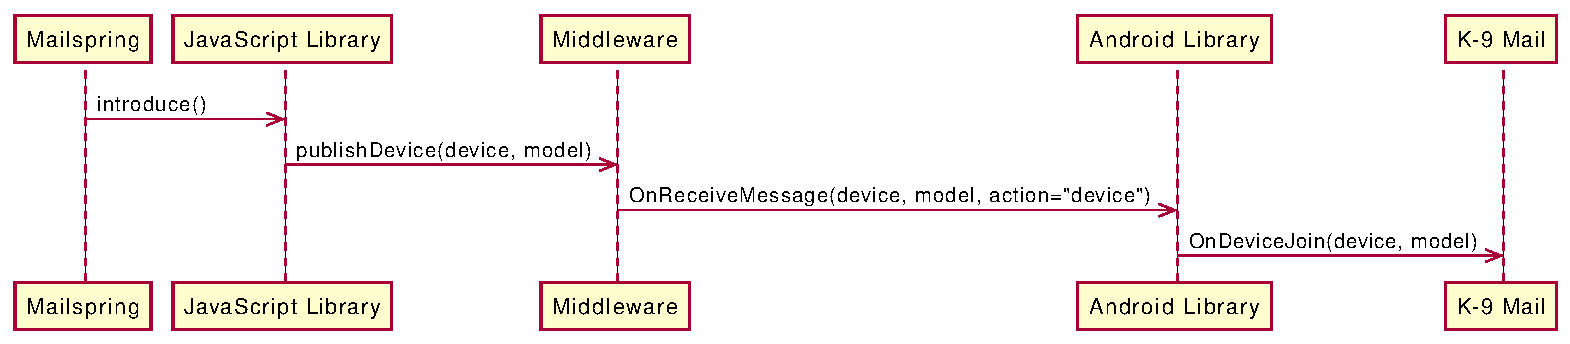
\includegraphics[width=\linewidth]{../figures/Initializing-Mailspring}
    \centering
    \caption{Initializing: Mailspring}
    \label{fig:Initializing-Mailspring}
\end{figure}

\subsection{Run-time State Management}
\subsubsection{Store State}
\begin{figure}
    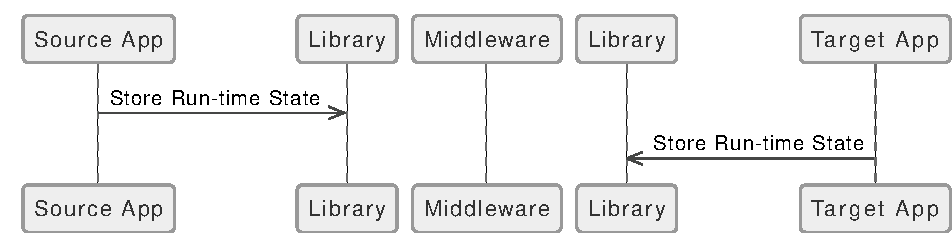
\includegraphics[width=\linewidth]{../figures/Store-Current-State}
    \centering
    \caption{Store the Current State}
    \label{fig:Store-Current-State}
\end{figure}
\subsubsection{Has State}
\begin{figure}
    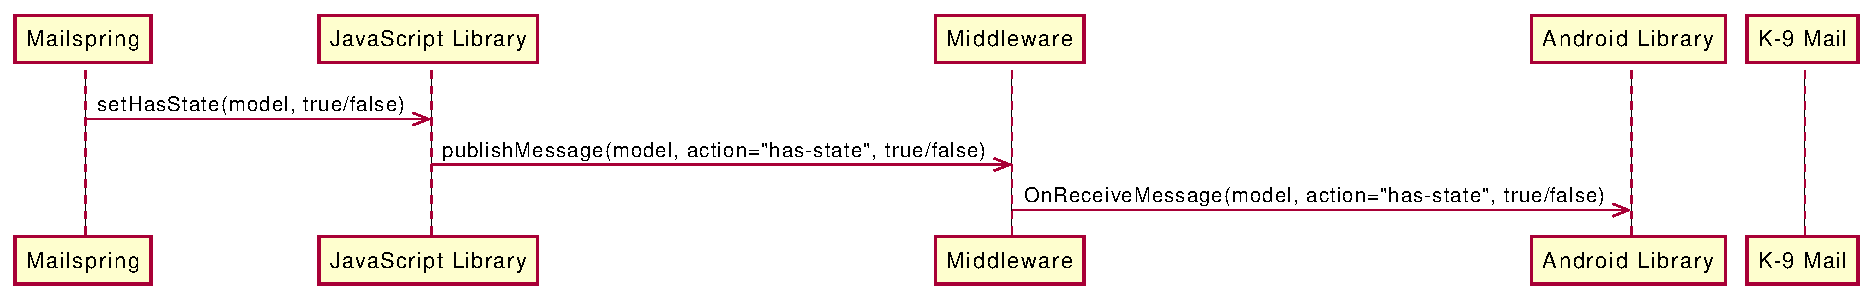
\includegraphics[width=\linewidth]{../figures/Inform-Devices-Has-State-Mailspring}
    \centering
    \caption{Inform other devices has a State: Mailspring}
    \label{fig:Inform-Devices-Has-State-Mailspring}
\end{figure}

\subsection{Migration Patterns}
\subsubsection{Pull Method}
\begin{figure}
    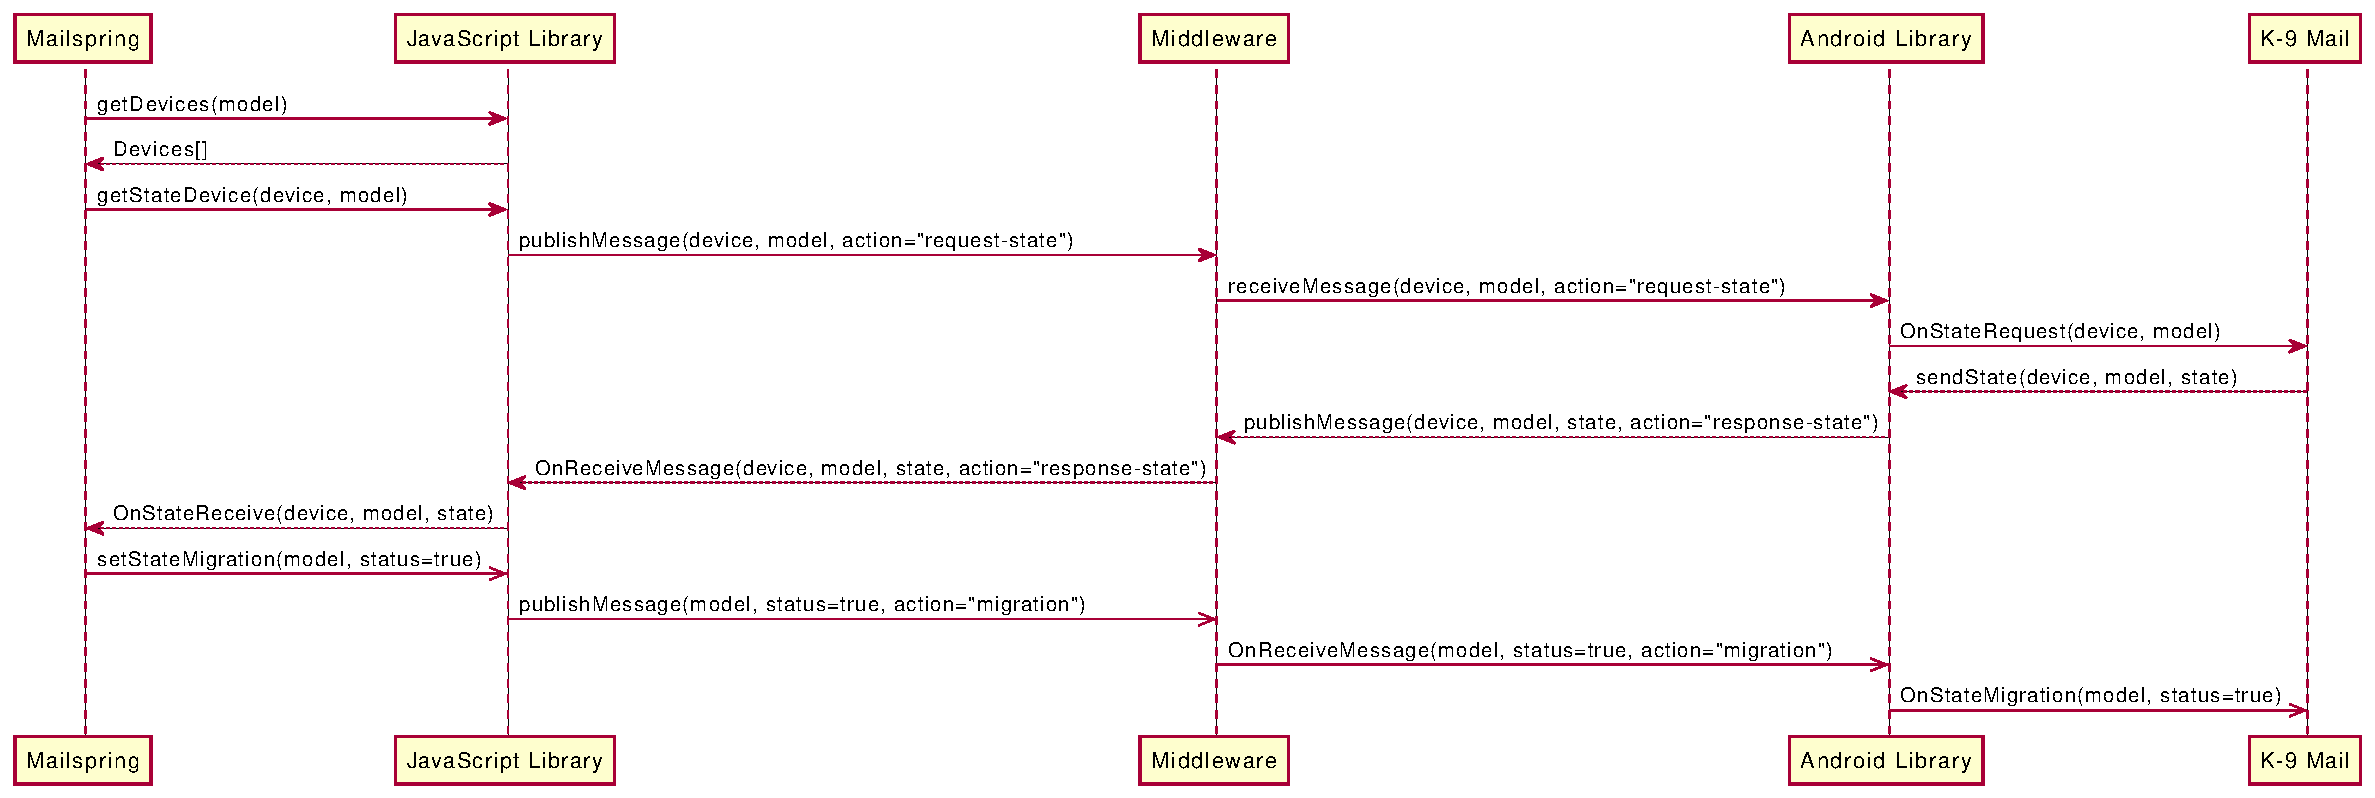
\includegraphics[width=\linewidth]{../figures/Migration-Mailspring-to-K9-Pull-Method}
    \centering
    \caption{Pull Method: Migration Mailspring to K9}
    \label{fig:Migration-Mailspring-to-K9-Pull-Method}
\end{figure}

\subsubsection{Push Method}
\begin{figure}
    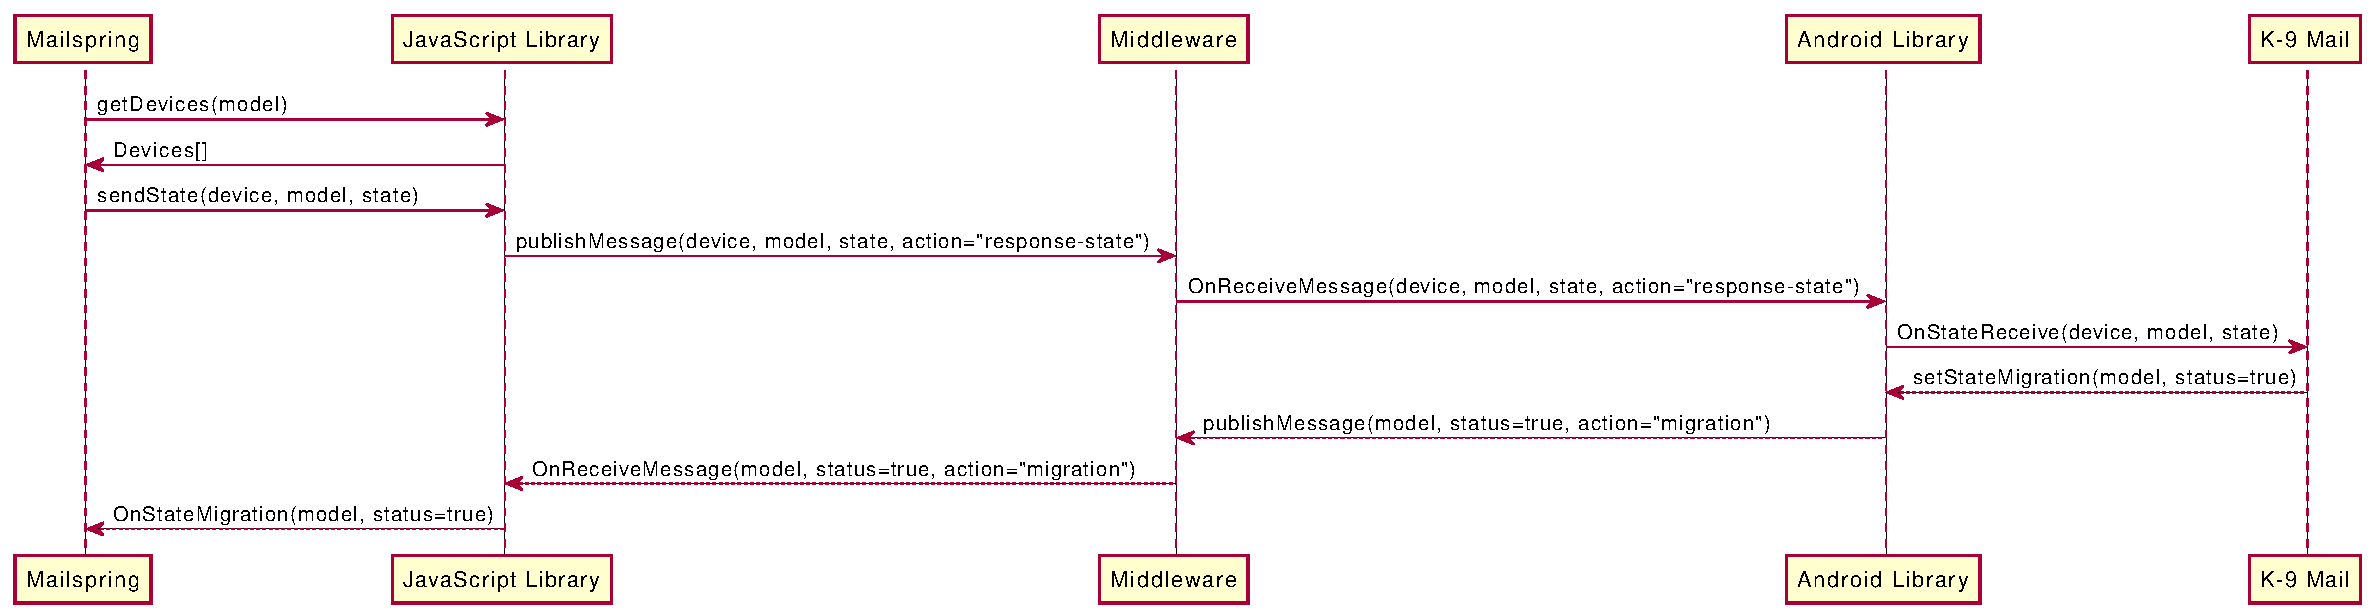
\includegraphics[width=\linewidth]{../figures/Migration-Mailspring-to-K9-Push-Method}
    \centering
    \caption{Push Method: Migration Mailspring to K9}
    \label{fig:Migration-Mailspring-to-K9-Push-Method}
\end{figure}

\subsection{Going Offline}
\subsubsection{Graceful}
\begin{figure}
    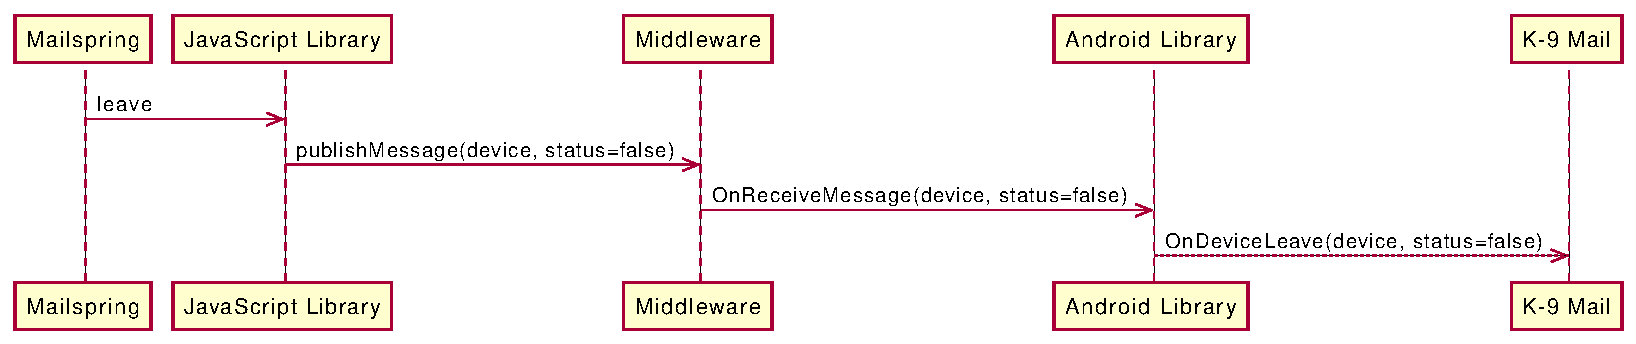
\includegraphics[width=\linewidth]{../figures/Going-Offline-Graceful-Mailspring}
    \centering
    \caption{Going Offline Gracefully: Mailspring}
    \label{fig:Going-Offline-Graceful-Mailspring}
\end{figure}
\subsubsection{Ungraceful}
\begin{figure}
    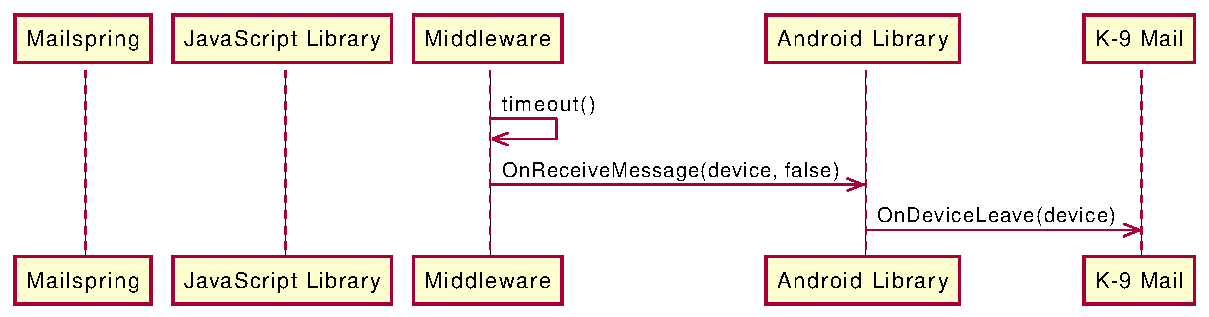
\includegraphics[width=\linewidth]{../figures/Going-Offline-Ungraceful-Mailspring}
    \centering
    \caption{Going Offline Ungracefully: Mailspring}
    \label{fig:Going-Offline-Ungraceful-Mailspring}
\end{figure}

\section{Helper Tools}
\subsection{ASML Schmea Library}
A repository which contains last est version of ASML JSON Schema files.

https://www.npmjs.com/package/asml

\subsection{ASML Editor}
an editor that developers can play with the ASML and ASM and RSM live.

https://asml-lang.github.io/asml/editor/

\subsection{ASML Validator Library}
a library to validate the DSL, which it used in asml-cli and rsm-node.

https://www.npmjs.com/package/asml-validator

\subsubsection{Installation}
\subsubsection{API}
\subsubsection{Usage}